\begin{frame}{3D Surface Plot}
\begin{center}
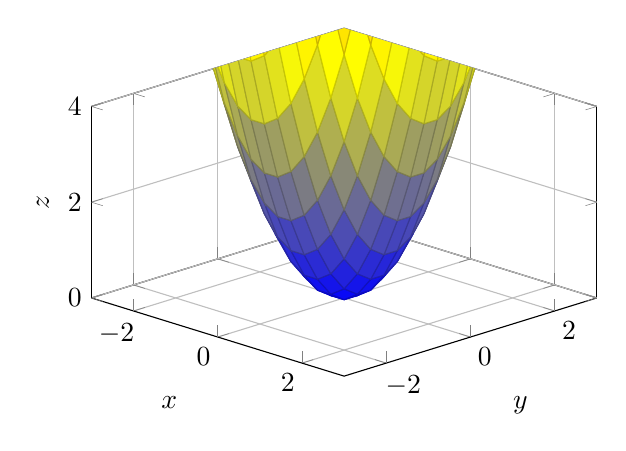
\begin{tikzpicture}
\begin{axis}[
    xlabel={$x$},
    ylabel={$y$},
    zlabel={$z$},
    grid=both,
    xmin=-3, xmax=3,
    ymin=-3, ymax=3,
    zmin=0, zmax=4,
    width=8cm,
    height=6cm,
    view={45}{30}
]
\addplot3[surf, domain=-3:3, samples=20] {x^2 + y^2};
\end{axis}
\end{tikzpicture}
\end{center}

\footnotesize
\texttt{\textbackslash addplot3[surf, domain=-3:3, samples=20] \{x\textasciicircum 2 + y\textasciicircum 2\};}
\end{frame}